\chapter{证明器的总体设计}
\label{chap:struct}
本章给出证明器的总体设计,并说明证明器的各个部分之间如何协作证明一个命题。

\section{输入语言}
本文设计的证明器需要证明的命题可以分成两部分:一部分是纯的一阶逻辑及其理论,另一部分是分离逻辑。前者主要表达程序中变量、函数之间的相等和不等关系,后者主要表示程序中数据结构的变化。

两者在各自推理的同时,前者也为后者服务,如向后者提供指针运算、指针相等关系等内容。这决定了证明器要支持一阶逻辑中的算术理论和相等理论。

由上述需求,我们设计的命题语言如图\ref{struct:syntax}所示。

\begin{figure}[!htbp]
  \centering
  \begin{tabular}{rrcl}
    整数常元 & $C$ & \sep & $\left\{ 0, 1, -1, \ldots \right\}$ \\
    整型变元 & $X$ & \sep & $\left\{ x_0, x_1, x_2, \ldots \right\}$ \\
    未解释函数 & $F$ & \sep & $\left\{ f_0, f_1, f_2, \ldots \right\}$ \\
    命题变元 & $A$ & \sep & $\left\{ A_0, A_1, \ldots \right\}$ \\
    公式项  & $T$ & \sep & $C$ \deli{} $X$ \deli{} $A$ \deli{} $F(T,$\ldots$,T)$ \deli{} $+(T, T)$ \deli{} $\cdot(C,T)$ \\
    一阶逻辑原子公式 & $Y$ & \sep{} & $T \le T$ \deli{} $T = T$ \deli{} $A$ \deli{} $\mathrm{true}$ \\
    一阶逻辑公式 & $\Pi$ & \sep{} & $Y$ \deli{}  $\lnot \Pi$ \deli{} $\Pi \impl \Pi$ \deli{} $\Pi \land \Pi$ \deli{} $\Pi \lor \Pi$ \\
    分离逻辑原子公式 & $H$ & \sep{} & $T \mapsto T$ \deli{} $\mathrm{emp}$ \\
    分离逻辑公式 & $\Sigma$ & \sep{} & $H$ \deli{} $\Sigma \ast \Sigma$ \\
    命题 & $P$ & \sep & $ \Pi \land \Sigma \impl \Pi' \land \Sigma' $
  \end{tabular}
  \caption{命题语言的语法}
  \label{struct:syntax}
\end{figure}

证明器接受的命题的整体是一个蕴含式,前件和后件都分别由$\Pi$和$\Sigma$两部分构成,分别代表一阶逻辑部分和分离逻辑部分。

$\Pi$和$\Pi'$是一个无量词的一阶逻辑公式。二元函数$+$和$\cdot$分别解释为整数环上的加法和数乘运算,这意味着只能支持线性的整数算术;除此之外,可出现有限个有限元的函数,它们是未解释的。

$\Sigma$和$\Sigma'$是包含分离逻辑符号的公式。为简化起见,分离逻辑公式只能用$\ast$(分离合取)联结词连接,原子公式只能是$\mathrm{emp}$和$T_1 \mapsto T_2$的形式,分别代表空堆和仅包含一项的堆。

命题语言语义的定义如图\ref{struct:semantic}。
\begin{figure}[!htbp]
  \centering
  \begin{tabular}{rcl}
    $s, h \models P$ & & \\
    $s$是栈 & & $s: T \impl \mathbb{Z}$ \\
    $h$是堆 & & $h: \mathbb{Z} 	\backslash \{0\} \impl \mathbb{Z}$ \\
    $s, h \models t_1 = t_2$ & $\iff$ & $s(t_1) = s(t_2)$ \\
    $s, h \models t_1 \leq t_2$ & $\iff$ & $s(t_1) \leq s(t_2)$ \\
    $s, h \models \mathrm{true}$ & $\iff$ & 真 \\
    $s, h \models \lnot P$ & $\iff$ & $s, h \models P$为假 \\
    $s, h \models P \impl Q$ & $\iff$ & 若$s, h \models P$,则$s, h \models Q$ \\
    $s, h \models P \land Q$ & $\iff$ & $s, h \models P$ 且 $s, h \models Q$ \\
    $s, h \models P \lor Q$ & $\iff$ & $s, h \models P$ 或 $s, h \models Q$ \\
    $s, h \models \mathrm{emp}$ & $\iff$ & $\mathrm{dom}(h)= \emptyset$ \\
    $s, h \models t_1 \mapsto t_2$ & $\iff$ & $s(t_1) \neq 0$ 且 $\mathrm{dom}(h) = \{s(t_1)\}$ \\
    & & 且 $h(s(t_1)) = s(t_2)$ \\
    $s, h \models P \ast Q$ & $\iff$ & 存在$h1, h2$, $h1 \bot h2$ 且 $h = h1 \ast h2$ \\
    & & 且 $s, h1 \models P$ 且 $s, h2 \models Q$ \\
  \end{tabular}
  \caption{命题语言的语义}
  \label{struct:semantic}
\end{figure}

由于分离逻辑隐式包含了堆,这在纯的一阶逻辑中是没有的。因此图中的语义定义主要说明了一阶逻辑符号拓展到有堆出现时的意义。

\section{证明项}
证明项是一种语言,它可以用来表示证明的推理过程。本文实现的证明器通过对每一个命题出具Coq兼容的证明项,来满足携带证明代码对携带机器可检查证明的要求。

\subsection{相关概念}
\subsubsection{Curry-Howard同构}
Curry-Howard同构\cite{HowardWA:fortnc}是指逻辑演算系统与程序类型系统的相对应关系。它指出,自然推理系统与$\lambda$-演算的对应关系如表\ref{tab:curry}。
\begin{table}[!ht]
  \label{tab:curry}
  \caption{自然推理系统与$\lambda$-演算的对应关系}
  \centering
  \begin{tabular}{cc}
    \whline
    自然推理 & $\lambda$-演算 \\
    \hline
    假设 & 对应类型的自由变量 \\
    蕴含引入 & 函数抽象 \\
    蕴含消去 & 函数应用 \\
    定理 & 对应类型的表达式 \\
    \whline
  \end{tabular}
\end{table}

于是,命题的证明问题就可以看作一个寻找对应类型的$\lambda$-表达式的过程。
例如,我们欲证明希尔伯特系统中的L1:
$$ \vdash P \impl (Q \impl P) $$

我们可以构造如下$\lambda$-表达式:
$$\lambda (H_0: P).(\lambda (H_1: Q).H_0)$$

上式的类型为$P \impl (Q \impl P) $,因此它是L1的一个证明。

\subsubsection{归纳构造演算与Coq}
归纳构造演算(Calculus of Inductive Constructions)是一种$\lambda$-演算的扩展,它结合了逻辑中的一些最新进展,因而能力更强。

Coq\cite{coq}是一个基于归纳构造演算的高阶逻辑定理证明辅助系统。其独到之处在于,表达程序和表达证明都使用同一套语言。

上一节L1的证明用Coq证明项表达如下:
\begin{verbatim}
    (fun H0:P => (fun H1:Q => H0))
\end{verbatim}

\subsection{表达证明项的数据结构}
我们将证明项保存为一个类似$\lambda$-表达式的形式。

证明项类型叫做\texttt{proof},定义用类ML语言描述如下:
\begin{verbatim}
    type param = (string * prop)        (* 参数 *)
    type proof =
    | Hole                               (* 空 *)
    | Id of string      (* 公理、定理、变量标识 *)
    | Lam of param list * proof    (* 函数抽象 *)
    | App of proof list            (* 函数应用 *)
\end{verbatim}

\texttt{Lam}和\texttt{App}构造分别模拟$\lambda$-表达式的函数抽象和函数应用。唯一不同的是,参数部分都被扩展成了列表,以更加便于实际使用。

\texttt{Hole}代表空,意味着没有找到命题的证明。

\texttt{proof}并不能表达纳构造演算的所有构造,但是在本文设计的证明器是足够用的。

\section{结构及流程}

\begin{figure}[!htbp]
  \centering
  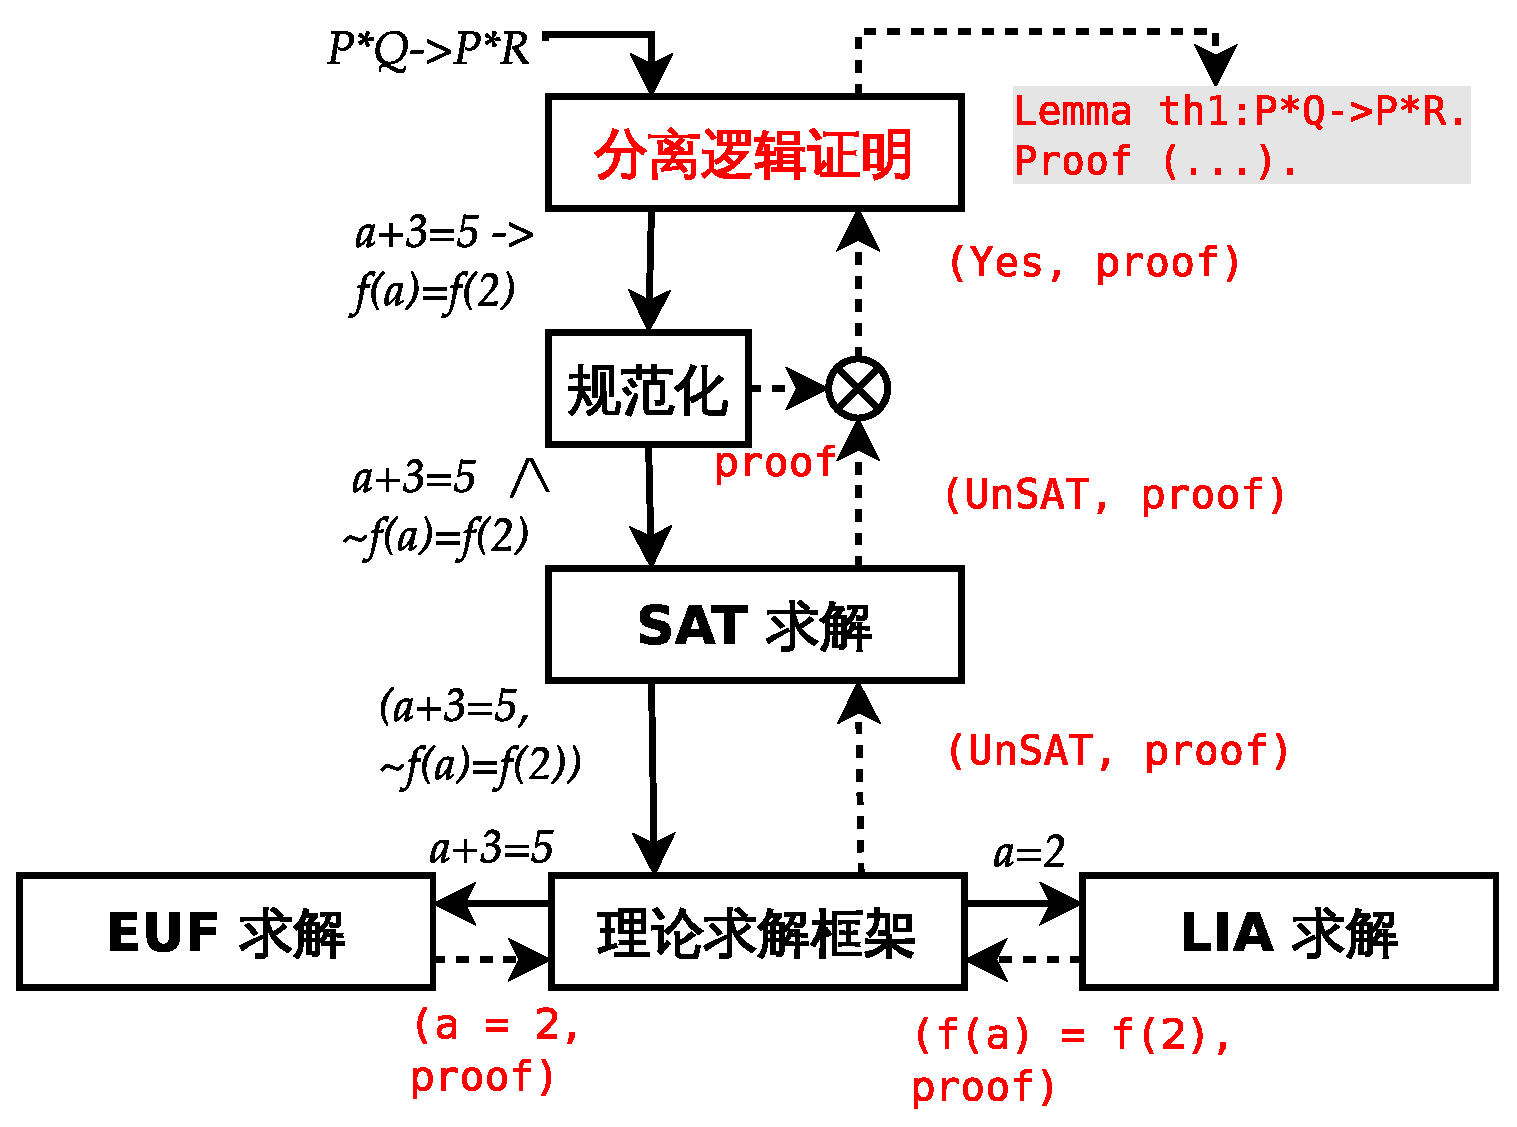
\includegraphics[width=0.8\textwidth]{stru.eps}
  \caption{证明器的结构}
  \label{struct:fig}
\end{figure}

如图\ref{struct:fig}所示,证明器逻辑上可以分成两大部分。一部分是传统的基于一阶逻辑的证明器;另一个部分是分离逻辑的证明器。

\subsection{分离逻辑的证明器所做的工作}
证明器开始运行时,接收命题语言$\Pi \land \Sigma \impl \Pi' \land \Sigma'$。

这个命题的证明可以化为求证:
\begin{eqnarray}
  \vdash & \Pi \land \Pi'' \impl \Pi' \label{struct:eq1}\\
  \vdash & \Pi \land \Sigma \impl \Sigma' \label{struct:eq2}
\end{eqnarray}

\ref{struct:eq1}式是一个纯的一阶逻辑的证明过程,因此直接将该部分命题发送到一阶逻辑的证明器求证。其中$\Pi''$是分离逻辑部分中推出的一些算术信息,如关于指针非空和不同堆的地址不同。

\ref{struct:eq2}式是一个带分离逻辑的证明过程。该部分将由分离逻辑的证明器使用分离逻辑中的定理将该过程分解成求证一系列纯一阶逻辑命题,并发送到一阶逻辑的证明器求证。该部分的方法在第\ref{chap:sep}章说明。

分离逻辑的证明器综合两式,得到命题的最终证明。

\subsection{一阶逻辑的证明器所做的工作}
一阶逻辑的证明器结构属于目前较先进的SMT(Satisfiability Modulo Theories)证明器结构。

对于每一个被发送到一阶逻辑的证明器的命题,首先经过命题逻辑证明模块。该模块将所有不同的公式项看作一个独立的命题变元,最终化简成为约束满足(SAT)问题,该步的具体方法在第\ref{chap:sat}章说明。

由于命题逻辑证明求解时不会关心命题公式项的具体内容,因此它在求解时会生成一系列可能否证命题的``反例''赋值。这些``反例''重新构成命题后被发送到理论整合框架。在这个框架中,命题被按照公式项分成不同的部分,送给不同的理论求解器求解。由于考察公式项的具体结构,``反例''将被一一反驳。该步具体方法在第\ref{chap:euf}、\ref{chap:lia}、\ref{chap:no}章说明。

命题逻辑证明模块综合这些反驳信息,得到一阶逻辑命题的最终证明。
